\section{Cours 10}\label{cours-10}

\subsection{La mémoire}\label{la-muxe9moire}

Accéder à la mémoire directement n'est pas une bonne solution car on
doit connaitre son organisation à la compilation. Impossible car si on
passe de 2 Go de RAM à 4 il faut tout recompiler !! On va virtualiser
tout ça

\subsubsection{La Mémoire Virtuelle}\label{la-muxe9moire-virtuelle}

On va devoir faire une traduction du virtuelle à physique via le
\textbf{MMU} ou \textbf{Memory Management Unit} (qui est dans le
processeur).

\begin{figure}
\centering
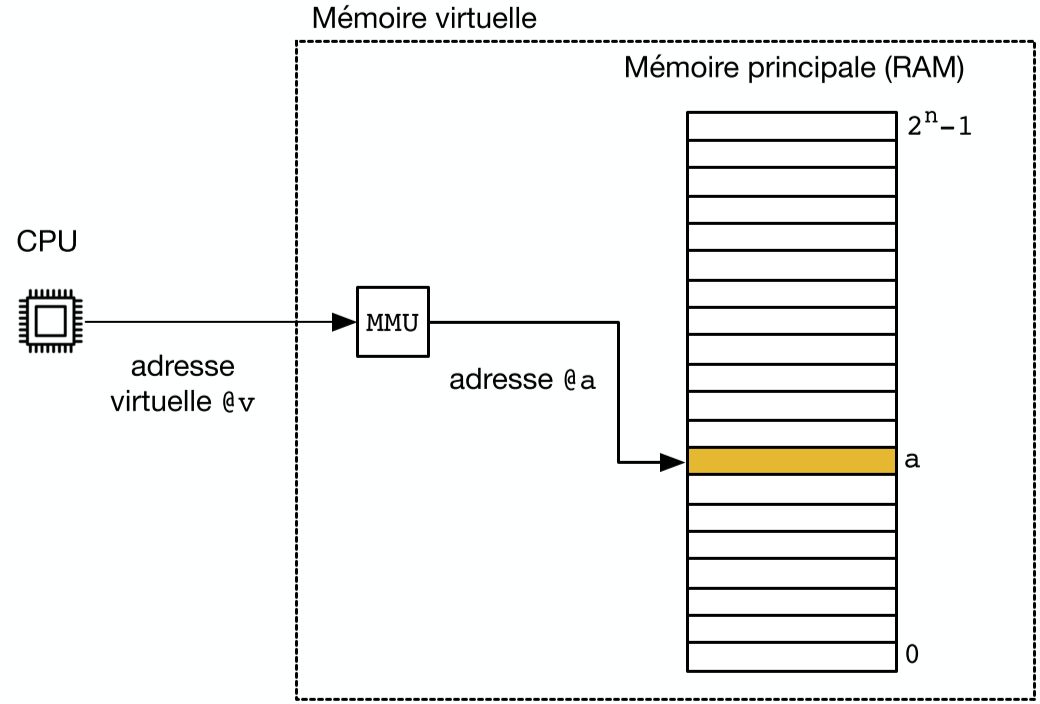
\includegraphics{image-52.png}
\caption{MMU Simple}
\end{figure}

Ainsi on peut découpler la taille et écrire les adresses sur + de 32
bits.

On peut faire de la librairie partagée très facilement, on peut voir que
2 programmes pointes vers la même zone de la RAM !

\paragraph{Avantages}\label{avantages}

On peut utiliser le stockage sur le disque pour mettre des objets
inutilisées de la RAM. C'est le principe de \textbf{\texttt{swap}}. Et
on peut faire vice-versa.

\subsubsection{Fonctionnement de la mémoire
Virtuelle}\label{fonctionnement-de-la-muxe9moire-virtuelle}

La mémoire a un accès par \emph{adresse} et les SSD par \emph{secteur}.
La mémoire virtuelle est divisée par \textbf{pages}. C'est une zone de
mémoire \textbf{contiguë} de taille 4 Ko (4096 octets (on peut vérifier
via \texttt{getpagesize()})).

On a toujours un nombre entier de pages. De plus, chaque segment (les 6)
occupe leurs propres pages.

Ainsi, les pages virtuelles peuvent être placées dans n'importe quelle
zone (\emph{frame}/cadre de page) de la mémoire physique.

Adresse Virtuelle est composée de:

\begin{itemize}
\tightlist
\item
  Numéro de la page
\item
  Offset sur cette page à faire
\end{itemize}

Le MMU se charge de la traduction.

\begin{figure}
\centering
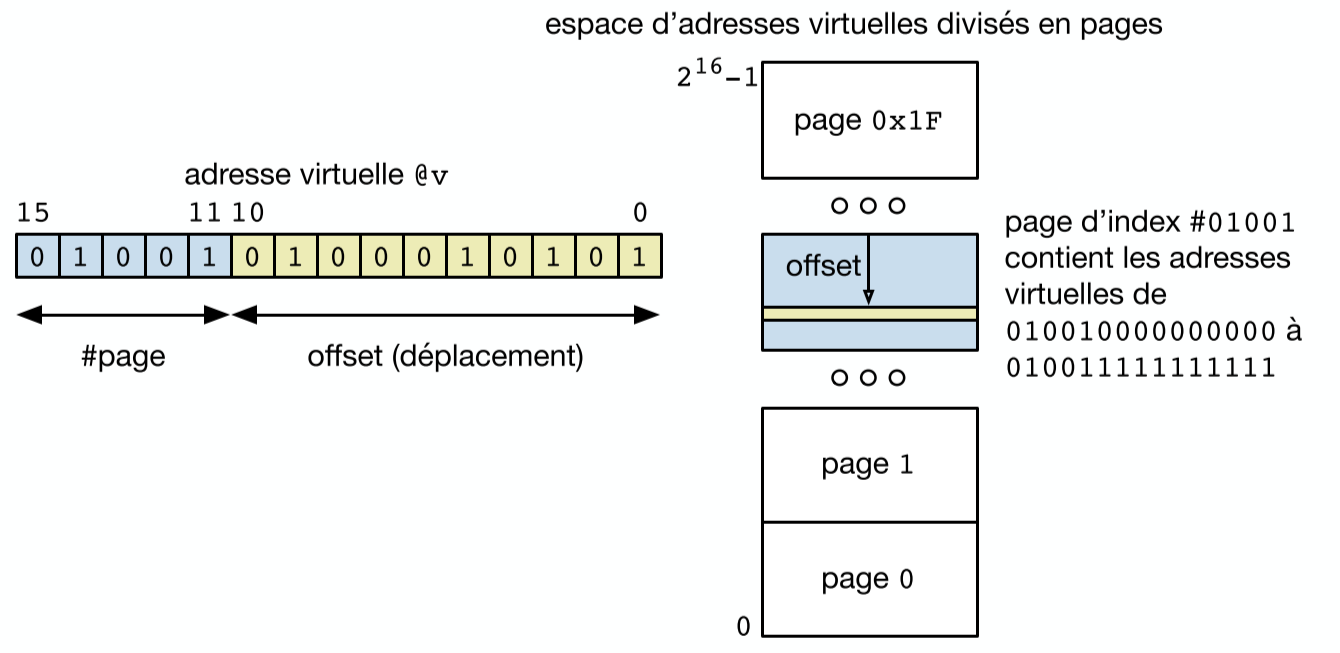
\includegraphics{image-53.png}
\caption{Découpage en page}
\end{figure}

\subsubsection{Mise en Oeuvre de la
Traduction}\label{mise-en-oeuvre-de-la-traduction}

Il doit avoir accès à l'allocation actuelle entre pages virtuelles et
cadres de pages physique. On va utiliser une table des pages:

\begin{itemize}
\tightlist
\item
  Tableau indexé par le numéro de page
\item
  Bit de validité si la page existe dans l'espace mémoire du
  \emph{processus}
\item
  Si valide: ligne du tableau indique le lien vers le numéro de cadre de
  page.
\end{itemize}

\begin{figure}
\centering
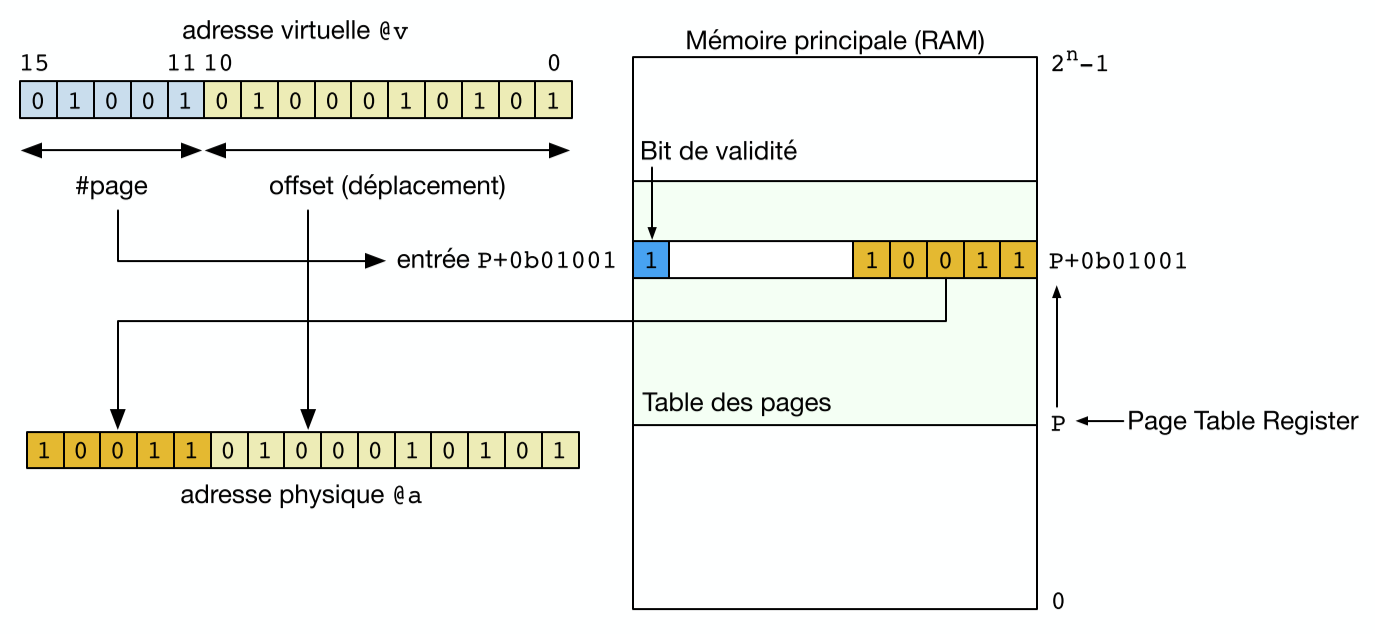
\includegraphics{image-54.png}
\caption{Traduction}
\end{figure}
